% ===== INICIO DEL PREÁMBULO =====
%
\documentclass[msc,oneside]{udelar} % Poner msc para Maestría, dsc para Doctorado.
%
\usepackage[
acronyms, 											 % Utiliza el glosario de acronimos.
nohypertypes={acronym,notacion,simbolos,glosario},   % Quita los links en el texto al glosario.
%nonumberlist,                                       % Quita los links en los glosarios al texto.
nogroupskip,                                         % Quita los espacios entre diferentes grupos dentro de un glosario.
nopostdot 											 % Quita el punto final en los acrónimos.
]{glossaries}

\hypersetup{ colorlinks = true } % Hipervínculos: escribir "false" para imprimir o "true" para ver en digital.

% Cargar estilo bibliográfico copiando del documento "Estilos bibliográficos UdelaRTeX.pdf"
\usepackage[style=ieee]{biblatex}
\usepackage{estilos_bibliograficos/udelartex_apa}

%\addbibresource{bibliografia/biblio_1.bib} % Agregar la cantidad de archivos .bib que se tengan para la bibliografía.
\addbibresource{bibliografia/biblio_2.bib} % Se coloca una línea por archivo .bib.

\loadglossary % No comentar esta línea

% A su vez, la clase udelar.cls ya tiene los siguientes paquetes cargados automáticamente, que podrían ser de interés saber para el usuario:
%{color},{hyphenat},{appendix},{lastpage},{babel},{inputenc},{amsmath,amssymb},{ifthen},{graphicx},{caption}{setspace},{tabularx},{eqparbox},{ltxcmds},{titletoc},{xcolor},{lineno},{xwatermark}

% Si se quieren agregar más paquetes, se recomienda colocarlos a partir de esta linea y antes de \begin{document}.
% ===========  INICIO PAQUETES ===============

% ===========   FIN PAQUETES   ===============


% =====  FIN DEL PREÁMBULO  =====

% ===== INICIO DEL DOCUMENTO =====

\begin{document}
  %
  \title{Aprendizaje profundo aplicado a problemas de calidad de datos}
  \subtitle{Utilización de autoencoders para medir la consistencia}
  \institutelogo{2} % Carga cantidad de logos seleccionados, con máximo de 3 logos. Si se pone un logo horizontal, colocar 1 o 2 logos para no desconfigurar la portada.
  \author{Ing. Andrés}{Veiro}
  \escritura{en} % Se indica que el programa de Posgrado sea "en" o "de" tal área.
  %
  \director{Prof.}{Adriana}{Marotta}{Dra.}
  %\director{Prof.}{Nombre del Director de Tesis}{Apellido}{D.Sc.}  Comentar esta línea si se tiene solo un director de tesis.
  %\codirector{Prof.}{Nombre del 1er Codirector}{Apellido}{D.Sc.}   Comentar estas líneas si no son necesarias.
  %\codirector{Prof.}{Nombre del 2do Codirector}{Apellido}{D.Sc.}
  %\codirector{Prof.}{Nombre del 3er Codirector}{Apellido}{D.Sc.}
  \directoracademico{Prof.}{Adriana}{Marotta}{Dra.}
  %
  \examiner{Prof.}{Nombre del 1er Examinador}{Apellido}{D.Sc.}
  \examiner{Prof.}{Nombre del 2do Examinador}{Apellido}{Ph.D.}
  \examiner{Prof.}{Nombre del 3er Examinador}{Apellido}{D.Sc.}
  \examiner{Prof.}{Nombre del 4to Examinador}{Apellido}{Ph.D.}
  \examiner{Prof.}{Nombre del 5to Examinador}{Apellido}{Ph.D.} % Comentar los que no son necesarios.
  %
  \graduatename{Sistemas de información y tecnologías de gestión de datos}
  \institute{Facultad de Ingeniería}{FIng}  % La primer institución es la principal.
  %\institute{Facultad de Medicina}{FMed}  % Agregar copias de esta línea para agregar instituciones.
  %\institute{Facultad de Agronomía}{FAgro}  % Agregar copias de esta línea para agregar instituciones. No se discrimina de que universidad es tal facultad.
  %\seconduniversity{Universidad XXXXX} % Se agrega el nombre de otra universidad. Comentar esta linea si no es necesaria.
 % \thirduniversity{Universidad YYYYY} % Se agrega el nombre de otra universidad. Comentar esta linea si no es necesaria.
  \graduatelocation{Montevideo}{Uruguay}
  %
  \date{01}{05}{2023} % Fecha del documento: día/mes/año
  % Palabras claves en español
  \keyword{Calidad de datos}
  \keyword{Aprendizaje automático}
  \keyword{3ra palabra clave}
  \keyword{4ta palabra clave}
  \keyword{5ta palabra clave}
  % Palabras claves en inglés
  \foreignkeyword{Calidad de datos}
  \foreignkeyword{Aprendizaje automático}
  \foreignkeyword{3rd keyword}
  \foreignkeyword{4th keyword}
  \foreignkeyword{5th keyword}
  %     
  \maketitle  % Comando que genera el título de la tesis.
  %
  \frontmatter  % Comando que genera la portadilla, el catalogo y el tribunal de evaluación. NO COMENTAR
  %
  \dedication{(Dedicatoria) A alguien cuyo valor es digno de ella.}


  \chapter*{Agradecimientos}

Quisiera agradecer a...

  \epigrafe{{\normalfont{(Epígrafe:)}} Frase que alude al tema de trabajo.}{Autor}


  \begin{abstract}

En esta tesis se presenta...

\end{abstract}


  \begin{foreignabstract}

 Property Graph databases are being increasingly used within the industry as a powerful and flexible way to model real-world scenarios. With this flexibility, a great challenge appears regarding profiling tasks due to the need of adapting them to these new models while taking advantage of the Property Graphs particularities. This work proposes a set of data profiling tasks by integrating existing methods and techniques, and an taxonomy to classify them. In addition, an application pipeline is provided while a formal specification of some tasks is defined.
\end{foreignabstract}
  %
%  \listoffigures	         % Lista de figuras
%  \listoftables	         % Lista de tablas
  \listadesimbolos 		 % Lista de símbolos
  \listadenotaciones 	     % Lista de notaciones
  \listadesiglas 		     % Lista de siglas
  %
  \tableofcontents           % Tabla de contenidos. Compilar dos veces para ver los cambios completos.
  %
  \mainmatter % Comando que genera las listas y capítulos. NO COMENTAR
  % 
  % Se incluyen los capítulos. Se pueden comentar los capítlos en los cuales no se está trabajando, para que el documento de trabajo sea más pequeño y compile más rápido.
  \include{capitulos/chap01}	% Se carga el capítulo 01
  \chapter{Fundamentos teóricos}

Este capítulo incluye la revisión de la literatura, de los enfoques, teorías o conceptos pertinentes en que se fundamenta la investigación. Se basa fundamentalmente en la exposición de otros trabajos sobre el tema estudiado.

En diferentes tradiciones académicas este capítulo recibe distintas denominaciones: Marco teórico, Estado de la cuestión, Estado del arte. El objetivo de este capítulo es guiar al lector en la interpretación de trabajos que se han ocupado previamente de la cuestión central de la tesis u ofrecen herramientas analíticas o interpretativas. 

Algunas disciplinas incluyen aquí objetivos, hipótesis y justificación de la metodología, en tanto que otras exigen capítulos independientes para estos contenidos. Asimismo, algunos trabajos requieren un capítulo propio para los antecedentes de la investigación.



\section{XXXX}

Es usual que en \textit{Fundamentos teóricos} o en otras partes de la tesis el autor incluya vocabulario específico de la disciplina en un glosario.

Un glosario incluye una lista de términos y su explicación sucinta. El objetivo de este apartado es permitirle a un lector especializado en el área, aunque no necesariamente en la temática, comprender con mayor facilidad ciertos términos. 
Se organiza en forma alfabética y en el cuerpo de la obra se lo puede señalar con \textsc{versalita} la primera vez que se menciona, si este tipo de letra no fue utilizado con otro fin.

Se mencionan a modo de ejemplo tres posibles palabras a definir:
%
\begin{itemize}
\item \gls{adjetivo}
\item \gls{adjetivo_re}
\item \gls{adjetivo_cu}
\end{itemize}
	% Se carga el capítulo 02
  \chapter{Metodología}

El objetivo de este capítulo es justificar el diseño metodológico elegido. La finalidad de una metodología bien descrita es explicitar los pasos mediante los cuales se obtienen los resultados, y por tanto el cumplimiento (o no) de los objetivos establecidos, de manera tal que pueda ser replicado por otro investigador. Si corresponde, también se evaluarán problemas metodológicos y se realizarán consideraciones éticas.
En algunas disciplinas este capítulo se denomina Materiales y métodos. 
En caso de que la investigación sea de carácter experimental, se debe especificar la siguiente información:


\begin{itemize}
\item	el tipo de investigación realizada (experimental, descriptiva, estudio de caso, encuesta de opinión, etc.)
\item	el modo de recolección de datos (análisis documental, observación participante o no, entrevista o cuestionario, etc.)
\item	población o sujetos experimentales.
\item	protocolo de investigación, si corresponde  
\end{itemize}

En algunas disciplinas formales no es pertinente la inclusión de un capítulo que recoja una cierta metodología de trabajo. En tales casos, se espera que el tesista haga mención de cuestiones carácter metodológico en la Introducción.

El procesamiento del trabajo metodológico que no es imprescindible para la comprensión del texto puede incluirse en apéndices o anexos (Anexo \ref{Ane1}).



	% Se carga el capítulo 03
  \chapter{Presentación de los datos, Análisis, Discusión}

En algunas disciplinas, el capítulo Presentación de datos va acompañado del análisis o de la discusión de la información (\textit{Presentación y análisis de los datos}; \textit{Resultados y discusión}), en tanto que en otras, \textit{Presentación}, \textit{Análisis} y \textit{Discusión} son capítulos separados.
El objetivo de esta(s) parte(s) de la tesis es presentar los datos recabados y el análisis realizado a la luz de la bibliografía ya revisada. Se puede incluir la interpretación de los resultados (\textit{Discusión}) a partir del análisis de los datos, o también relacionarlos con estudios relevantes que se entienden pertinentes, aun si estos no se han consignado en los \textit{Fundamentos teóricos}, ya que se entiende que al analizar los datos pueden aparecer algunos que no se enmarcan teóricamente o que no se explican en el encuadre teórico o en estudios ya existentes.

Ahora a modo de ejemplo mencionamos el símbolo de los números reales utilizando el comando \verb|\gls{}| \gls{Real} y el comando \verb|\glssymbol{}| \glssymbol{Real}. Otro ejemplo es mencionar el tensor simétrico de tensiones \gls{sigma}, o un valor escalar  \gls{alph} o un conjunto vacío \gls{emptyset}.

\newpage 


\section{Título de sección}

Ejemplo de tabla

\begin{table}[h!]
\centering
\caption{Leyenda de tabla.}
\label{tab:comp}
\begin{tabular}{|c|c|c|}
  \hline
  $t$ (seg) & $x$(t) & $y$(t)\\
  \hline
  1 & 0.0000 & 0.0001\\
  2 & 0.5000 & 0.2498\\
  3 & 1.0000 & 1.0000\\
  4 & 1.5000 & 2.2403\\
  5 & 2.0000 & 4.0010\\
  6 & 2.5000 & 6.2459\\
  \hline
\end{tabular}
\end{table}

Ejemplo de figura.

\begin{figure}[h!]
\label{fig:comp}
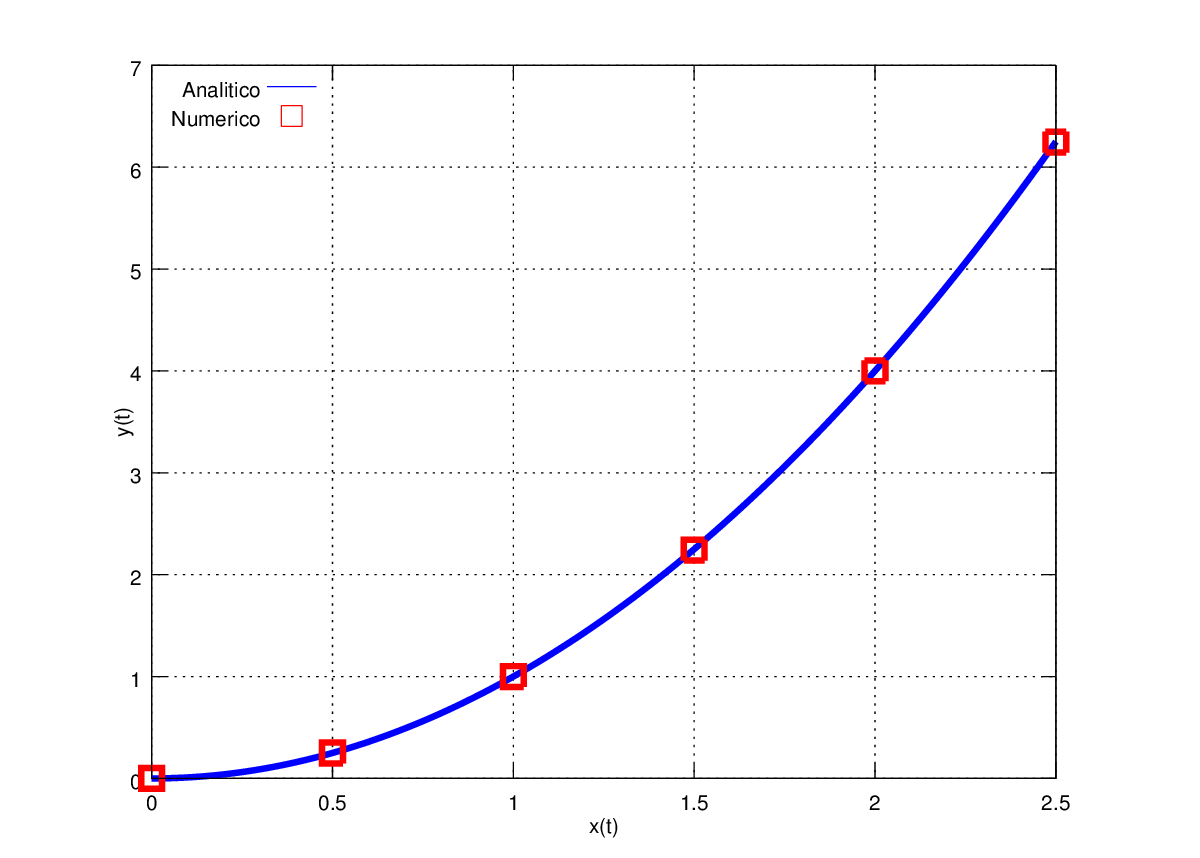
\includegraphics[width=.8\textwidth]{imagenes/chap4/x_vs_y}
\caption{Leyenda de figura.}
\end{figure}
Ejemplo de ecuación:
\begin{equation}
y(x)=x^2
\end{equation}
 	% Se carga el capítulo 04
  \chapter{Consideraciones finales}

 \cite{Batini} En este capítulo se sintetizan las posturas expuestas en el capítulo anterior. Se retoma la pregunta de investigación y se expresa si los resultados apoyan o no la hipótesis planteada. 

Además, se pueden hacer contribuciones teóricas o metodológicas a la disciplina y recomendaciones para trabajos futuros o para profundizar en el campo, plantear nuevas interrogantes o proponer explicaciones \textit{post hoc}. En algunos trabajos este capítulo se subdivide en otras secciones que presentan algunos de los contenidos mencionados. 
En algunas tradiciones académicas este capítulo recibe distintas denominaciones: \textit{Conclusiones}, \textit{Conclusiones y trabajos a futuro}, \textit{Consideraciones finales y recomendaciones}. 

 	% Se carga el capítulo 05

  % Seguir copiando la linea de arriba para agregar más capítulos.
  
  \backmatter % Comando que generalos apéndices, anexos y bibliografía. NO COMENTAR
  

  \printbibliography		% Se imprimen las referencias bibliográficas
  
  \bibend % NO comentar
  % 
  \glosario 		         % Glosario, NO comentar
  %
  \apenarabicnumbering
  \apenmatter				 % Apéndices, NO comentar
%  \chapter{Datos procesados}


%  \chapter{Imágenes remasterizadas}\label{Ape2}

%  \chapter{Entrevistas desgrabadas}\label{Ape3}

  % Seguir copiando la linea de arriba para agregar más apéndices.
  %
  \anexarabicnumbering
  \anexmatter				 % Anexos, NO comentar
%  \chapter{Material legislativo}\label{Ane1}

XXXXX
%  \input{anexo/anexo_B}
  % Seguir copiando la linea de arriba para agregar más anexos.
  % 
\end{document}

% ===== FIN DEL DOCUMENTO =====